\chapter{Fundamentos teóricos}

O desenvolvimento para sistemas embarcados necessita de uma interface para desenvolvimento do código fonte, um compilador para geração do código fonte para código de maquina e um sistema de carregamento do código de maquina para o sistema embarcado.

\section{Sistema embarcado}

Numa visão mais ampla, o sistema embarcado pode ser resumido para qualquer sistema que realiza uma tarefa especifica, independe do custo energético ou computacional\cite{barr2006programming}. Dentro desta categoria, pode-se listar alguns exemplos:

\begin{itemize}
\item \textbf{VANT} (Veículo Aéreo Não Tripulado) - Com crescimento exponencial nos últimos anos, atualmente se encontra com inúmeras propostas em suas utilizações.
\item \textbf{Roteador} - Extremamente populares no acesso da internet. Muitos contem uma arquitetura computacional completa , processador, memória e sistema operacional como o \textit{OpenWrt}\cite{openwrt}.
\item \textbf{GPS} (\textit{Global Positioning System}) - Com um sistema de processamento, podendo realizar filtragem, fusionamento, estimação e comunicação em inúmeros protocolos.
\item \textbf{Televisões} - Os modelos dos últimos anos tiveram como foco principal a extensão da televisão como ambiente de entretenimento, permitindo conexão com internet, instalação de aplicativos e serviços online de entretimento e informação.
\item \textbf{Câmeras de vigilância} - Alguns tipos permitem o acesso via internet, utilizando uma eletrônica embarcada com sistemas operacional e periféricos de rede.
\end{itemize}

\abreviatura{VANT}{\textit{Veículo Aéreo Não Tripulado}}
\abreviatura{GPS}{\textit{Global Positioning System}}

As definições de sistemas embarcados foram modificadas ao passar do tempo, como, por exemplo, o baixo processamento, que se tornou inapropriada ao passar dos anos\cite{aiimpacts}.

\iffalse
A evolução do hardware, diminuiu o tamanho e preço de aquisição dos processados, permitiu praticamente a qualquer desenvolvedor de
sistemas computacionais embarcados, um poder de processamento grande o suficiente para rodar um kernel\footnote{Cerne do sistema
operacional, tendo como principal função o escalonamento de tarefas e abstração dos periféricos de hardware utilizados da maquina,
como, por exemplo: placa de rede, sensores, portas de comunicação, \textit{GPIOs} e etc.} de sistema operacional complexo, como o Linux, em praticamente qualquer aplicação.

Muitas das aplicações de sistemas embarcados são utilizados para sistemas cyber-físicos\footnote{Sistemas computacionais
voltados para interação no mundo físico via atuadores e tendo como entrada informações de transdutores, alguns exemplos
podem se destacar: Controle de combustível, controladora de VANTs, impressora 3D e etc.}
\fi

\section{Distinção entre sistemas}
Dentro da área de sistemas embarcados, por envolver uma ampla gama de periféricos, utilizações, finalidades, pode-se resumir a certas categorias de destaque em relação a unidade principal de processamento, podendo destacar:

\subsection{Microcontrolador}

Um microcontrolador é definido como um sistema completo, sendo geralmente autossuficiente em relação aos periféricos necessários para realizar seu funcionamento. O processador, memória, periféricos de entrada e saída (\textit{ADC}, \textit{PWM}, \textit{GPIO}, entre outros) e oscilador na mesma pastilha de silício (\figref{fig:ricv}), barateando os custos de sua confecção, permitindo a popularização dos mesmos na industria e na comunidade DIY (Do It Yourself)/Makers\footnote{Cultura de desenvolvimento tecnológico próprio, derivado do movimento \textit{DIY}, sendo conhecido pela construção, modificação e manutenção pessoal.}. Estes mesmos
sistemas permitem o uso de osciladores externos, possibilitando o aumento da frequência de \textit{clock}\footnote{Sinal temporal periódico que determina a atualização dos registrados do sistema.} e como consequência um acréscimo no MIPS.

\abreviatura{DIY}{\textit{Do It Yourself}}
\abreviatura{SoC}{\textit{System on a chip}}
\abreviatura{ADC}{\textit{Analog to Digital Converter}}
\abreviatura{PWM}{\textit{Pulse Width Modulation}}
\abreviatura{GPIO}{\textit{General Purpose Input/Output}}
\abreviatura{DIY}{\textit{Do It Yourself}}
\abreviatura{MIPS}{Milhões de Instruções Por Segundo}

%https://twitter.com/onchipUIS/status/764289155983675392

\begin{figure}[!htb]
  \centering
  \caption[Microcontrolador na pastilha de silício.]{Microcontrolador 32 bits baseado na arquitetura \textit{RISCV} (\textit{Reduced Instruction Set Computing - V})\footnote{Arquitetura aberta baseada na \textit{RISC}.}
  com periféricos (\textit{ADC}, \textit{DAC} (\textit{Digital-to-Analog Converter}), \textit{GPIO} e memória \textit{RAM} (\textit{Random Access Memory})), Fonte: onchip\cite{onchip}.}
  \label{fig:ricv}
  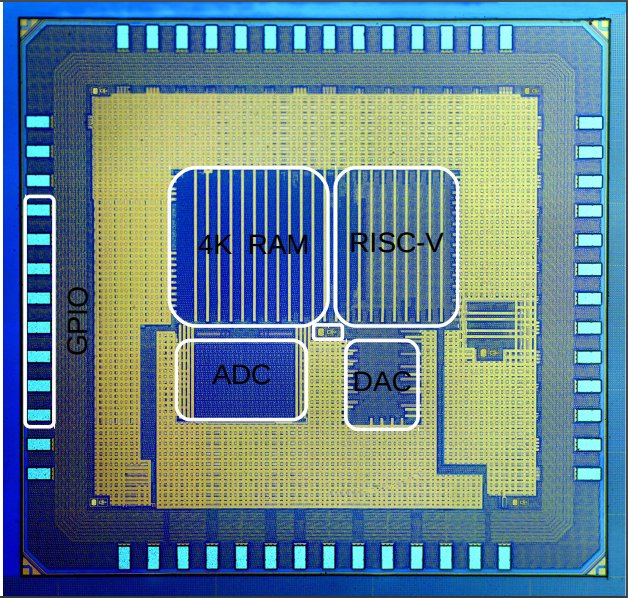
\includegraphics[width=0.5\textwidth]{figuras/riscv.jpg}
\end{figure}

\abreviatura{DAC}{\textit{Digital-to-Analog Converter}}
\abreviatura{RAM}{\textit{Random Access Memory}}
\abreviatura{RISCV}{\textit{Reduced Instruction Set Computing - V}}

Se nas ultimas décadas, o acesso a computadores se tornou facilitado, nas próximas que estão por vir, o uso e aquisição de sistemas computacionais não será um mero luxo, mas sim uma inevitabilidadea\cite{gates1995estrada}. Tudo terá um processador, se não, um sistema computacional simples. Pode-se notar muitas etiquetas de RFID (\textit{Rafio Frequency Identification}) e cada vez mais modernas \cite{ricci2008design}, contendo sistemas computacionais complexos.

\abreviatura{RFID}{\textit{Rafio Frequency Identification}}

\subsection{Microprocessador}

Parte principal de um sistema computacional, com o objetivo de decodificar e executar as instruções em código de maquina existente na memória\cite{Patterson:2008:COD:1502247}. A tabela que é interpretada, denominada por conjunto de instruções, contem todos os padrões binários possíveis a serem decodificados, resultando em sinais lógicos para a eletrônica que o executará, podendo realizar comparações, somas, multiplexações e leituras/escritas na memória.

Com o passar dos anos, o poder de processamento permitiu que sistemas simples possam ter grande valor intelectual agregado, podendo utilizar como exemplo o termostato da Google, vendido atualmente por \$250, por realizar um \textit{aprendizado de maquina}\footnote{"Campo de estudo que dá aos computadores a habilidade de aprender sem serem explicitamente programados`` -  Arthur Samuel, 1945.}, proporcionando ao aparelho um melhor gerenciamento da temperatura do ambiente, realizando uma economia energética e uma melhora na qualidade de vida do usuário.

\subsection{SoC}

Atualmente o termo é empregado a circuitos com uma vasta quantidade de sistemas integrados, podendo citar  \textit{GPU} (\textit{Graphics Processing Unit}), \textit{USB} (\textit{Universal Serial Bus}), módulos de rede, rádio e outros sistemas mais avançados.

\abreviatura{GPU}{\textit{Graphics Processing Unit}}
\abreviatura{USB}{\textit{Universal Serial Bus}}

Nesta categoria, pode-se destacar o desenvolvimento dos sistemas desenvolvidos pela fabricante ARM, tendo ultrapassado a Intel como a maior produtora de processamentos do mundo.
Após a revolução dos dispositivos móveis onde a maioria das pessoas começaram a utilizar \textit{smartphones}, acarretando na substituição do uso de computadores para realizar as suas rotinas pessoais digitais diárias. Esta revolução, está fazendo uma grande modificação no ambiente de desenvolvimento das grandes empresas, permitindo o desenvolvimento de hardware sem a necessidade de empresas altamente especializadas para desenvolvimento, tornando um foco de desenvolvimento genérico e macroscópico.


\section{Bootloader}

A vantagem de se utilizar um sistema de carregamento de boot\footnote{Processo no qual o sistema computacional se inicia.} é
a gravação do programa principal com a assistência de um software primário, conhecido como \textit{bootloader}. Um microcontrolador
com este sistema, também pode ser denominado de auto-programável, pois possui as dependências necessárias para realizar o próprio
processo de programação.

Para entender melhor o funcionamento, pode-se utilizar uma maquina de estados para detalhar o \textit{bootloader} utilizado nos microcontroladores AVR (\figref{fig:sm_bootloader}), e uma descrição dos estados na \tabref{tab:bootloader}.

\begin{figure*}[ht!]
  \centering
  \begin{tikzpicture}[->,>=stealth',shorten >=1pt,auto,node distance=2.8cm,
                      semithick]
    \tikzstyle{every state}=[fill=blue,draw=none,text=white]

    \node[inicio,state]  (A)                    {$init\_hw$};
    \node[state]         (B) [right of=A]       {$new\_prg$};
    \node[state]         (C) [below of=B]       {$get\_com$};
    \node[state]         (D) [left of=C]        {$chk\_com$};
    \node[state]         (E) [left of=D]        {$exe\_com$};
    \node[state]         (F) [right of=B]       {$run\_prg$};

    \path (A) edge              node {}      (B)
          (B) edge              node {sim}   (C)
              edge              node {não}   (F)
          (C) edge              node {}      (D)
          (D) edge              node {correto}      (E)
              edge [bend right] node [above] {erro} (C)
          (E) edge [bend right] node [below] {}     (C);
  \end{tikzpicture}
  \caption[Máquina de estados do avr \textit{bootloader}]{\label{fig:sm_bootloader}}{Máquina de estados
  do avr \textit{bootloader},\\Fonte: \textit{AVR109: Self Programming - ATMEL}.}
\end{figure*}

\begin{table}[ht!]
\centering
\caption[Descrição dos estados do \textit{bootloader}]{Descrição dos estados da \figref{fig:sm_bootloader}}
\label{tab:bootloader}
\begin{tabular}{@{}l l p{55mm}@{}}
\toprule
Estado             & Próximos estados           & Descrição                                                                                                             \\ \midrule
\textit{init\_hw}  & \textit{new\_prog}         & Inicializa depêndencias de hardware para a utilização do \textit{bootloader}, Ex: serial.                \\
\textit{new\_prog} & \textit{get\_com,run\_prg} & Espera uma interrupção de hardware ser inicializada para inicialização da rotina de \textit{bootloader}. \\
get\_com           & \textit{chk\_com}          & Adiquiri os dados do \textit{buffer} da serial.                                                                     \\
chk\_com           & \textit{exe\_com,get\_com} & Checa o comando recebido pela serial, caso o não é valido outro comando deverá ser buscado.                           \\
exe\_com           & \textit{get\_com}          & Executa o comando após a validação                                                                                    \\
run\_prg           &                            & Inicializa programa principal caso a rotina de programação não é inicializada via interrupção de hardware. \\ \bottomrule
\end{tabular}
\end{table}

O \textit{bootloader}, por ser uma peça de software essencial dos sistemas auto-programáveis, ele se encontra na parte da memória
não volátil, existindo dentro de uma faixa determinada da memória ao lado do programa principal que será executado, como pode ser
visualizado na \figref{fig:me_bootloader}.

\begin{figure*}[ht!]
  \centering
  \begin{bytefield}{11}
    \memsection{ffff ffff}{002f c000}{6}{Pilha}\\
    \begin{rightwordgroup}{Flash}
        \memsection{002f bfff}{0001 0000}{3}{Aplicação principal}\\
        \memsection{0000 ffff}{0000 0000}{2}{\textit{Bootloader}}
    \end{rightwordgroup}\\
  \end{bytefield}
  \caption[Memória com \textit{bootloader}]{\label{fig:me_bootloader}}{Memória com \textit{bootloader},\\Fonte: 
  \textit{``Modular bootloader framework for silicon labs SIMXXXXX microcontrollers - Silicon Labs''}.}
\end{figure*}

%\subsection{Gravação}
%O processo é a transmissão do novo código a ser enviado para a memória do sistema embarcado, r

%\itodo{[ADICIONAR  UMA LISTA DOS BOOTLOADERS]}

\section{Programação externa}
%é importante
A realização da programação externa, utilizando um hardware especializado que  permiti a programação do processador, independente do software que já está programado ou em execução.
Alguns processadores, que se encontram em estados indevidos ou não planejados, podendo acarretar no mal funcionamento do sistema, podem ser regravados sem a preocupação do \textit{bootloader}, utilizando a gravação com a ferramenta do hardware especializado, limpando toda a memória e gravando o programa. O mesmo também é necessário para realizar a gravação do \textit{bootloader} pela primeira vez no processador, após isso, o próprio \textit{bootloader} pode se reprogramar ou atualizar.

A programação via um hardware especializado é geralmente concebida, dentro dos softwares livres, com o OpenOCD (\textit{Open On Chip Debugger})\cite{openocd}, realizando a interface de software na comunicação com o hardware especializado como o JTAG (\textit{Joint Test Action Group}).

\abreviatura{JTAG}{\textit{Joint Test Action Group}}
\abreviatura{OpenOCD}{\textit{Open On Chip Debugger}}

\section{JTAG}

\section{KDevelop}
O plugin proposto foi desenvolvido sobre a plataforma conhecida como KDevelop,\cite{kdevelop} pertencente a organização \textit{KDE},
sendo um conceito de \textit{IDE} para programação.

Concebido utilizando as tecnologias de código aberto mais modernas, como C++14, QT 5.8, entre outras bibliotecas e ferramentas
utilizadas, podendo assim denominar o sistema como \textit{Rolling release}\footnote{Sistemas de software que atualizam suas bases
de código para a utilização das ultimas versões das ferramentas empregadas no projeto.}.

O \textbf{KDevelop} teve seu primeiro lançamento em 1999, sendo majoritariamente programado em C++, podendo ser utilizado
para programar em C, C++, Perl, Python, PHP, Java, Fortran, Ruby, Ada, Pascal, SQL e Bash. Suportando também sistemas de
configuração para compilação como cmake, qmake e make.

Diferente de outras \textit{IDEs} que propõem as mesmas soluções que o KDevelop, este é inteiramente desenvolvido
com foco em performance e numa agradável experiência do usuário, permitindo o desenvolvimento e adesão de projetos na \textit{IDE} (\textit{Integrated Development Environment}) sem restringir outros ambientes de desenvolvimento, utilizando toda a informação disponível nos sistemas assistencialistas de configuração de compilação, como fonte das dependências e de informações sobre o projeto adicionado. Para um programador comum de código aberto, o KDevelop se apresenta como uma ótima opção.

\abreviatura{IDE}{\textit{Integrated Development Environment}}

\subsection{Plugins}
O \textit{plugin} opera como uma biblioteca compartilhada que é carregada durante o tempo de execução, desta forma, providenciando acesso as funções da biblioteca. Uma grande vantagem da sua utilização é o uso modular das dependências utilizadas no projeto, sem a necessidade de ter o conjunto como um único binário com todas as dependências, mesmo aquelas não utilizadas pelo desenvolvedor.

Uma outra vantagem da utilização de \textit{plugins}, é permitir somente a utilização do binário, sem a necessidade de utilizar
o código fonte do mesmo, permitindo, a utilização de \textit{plugins} que não são de código aberto, facilitando desta
forma o apoio e uso de sistemas proprietários desenvolvidos, mantendo sigiloso o trabalho intelectual.

\subsection{Tipos de ferramenta}
Das ferramentas disponibilizadas para o desenvolvimento destas a Plicações possuem algumas limitações tais como, preço, licença, configuração entre outros, podendo ser classificadas conforme as seguintes categorias:

\begin{itemize}
 \item \textbf{Ferramentas proprietárias}: Ferramentas de desenvolvimento que geralmente utilizam software e hardware desenvolvido pelo próprio fabricante, não dando suporte a outros periféricos que não pertencem a mesma distribuidora ou parceira, limitando a liberdade de desenvolvimento. Outras permitem o desenvolvimento limitado para cada tipo de licença, dificultando o desenvolvimento que utilizam baixo orçamento, como, por exemplo: Limitação de tamanho de código\cite{simplicity}, pagar uma licença mais cara para utilizar opções de compilação otimizada (-O2 e -OS do GCC, C++11/14)\cite{armdeveloper} ou até mesmo opções para utilizar o algumas partes do processador (neon, -mfloat-abi e -mfpu dos processadores ARM, permitindo execução de cálculo matricial ou com ponto flutuante em hardware)\cite{neon}. A utilização de ferramentas proprietárias são majoritariamente usadas.

 \item \textbf{Ferramentas de código aberto}: Utilizadas por uma parte dos desenvolvedores, fornece acesso total as suas funcionalidades, possibilitando modificações e aperfeiçoamentos nos mínimos detalhes. Estas interfaces permitem o desenvolvimento com uma experiência mais assistencialista, por possuir uma comunidade grande de desenvolvedores que disponibiliza suporte por e-mail ou grupos de chat. Contudo, por estar em constante evolução, sua documentação pode estar defasada ou inexistente.

\end{itemize}

\section{Sistema de Controle de Versão}

Para o controle do projeto desenvolvido foi utilizado o \textit{GIT}, permitindo o controle de versão do código, paralelismo no desenvolvimento, detecção de conflitos entre diferentes versões, detecção de erros, entre outras utilizações de grande valia
para o desenvolvimento de software.

\abreviatura{GIT}{\textit{Global Information Tracker}}
